\section{RQ2: How Fast Does Observed State Expire?}
\label{sec:rq2}

\subsection{Two channels, one grid}
\begin{figure}[t]
\centering
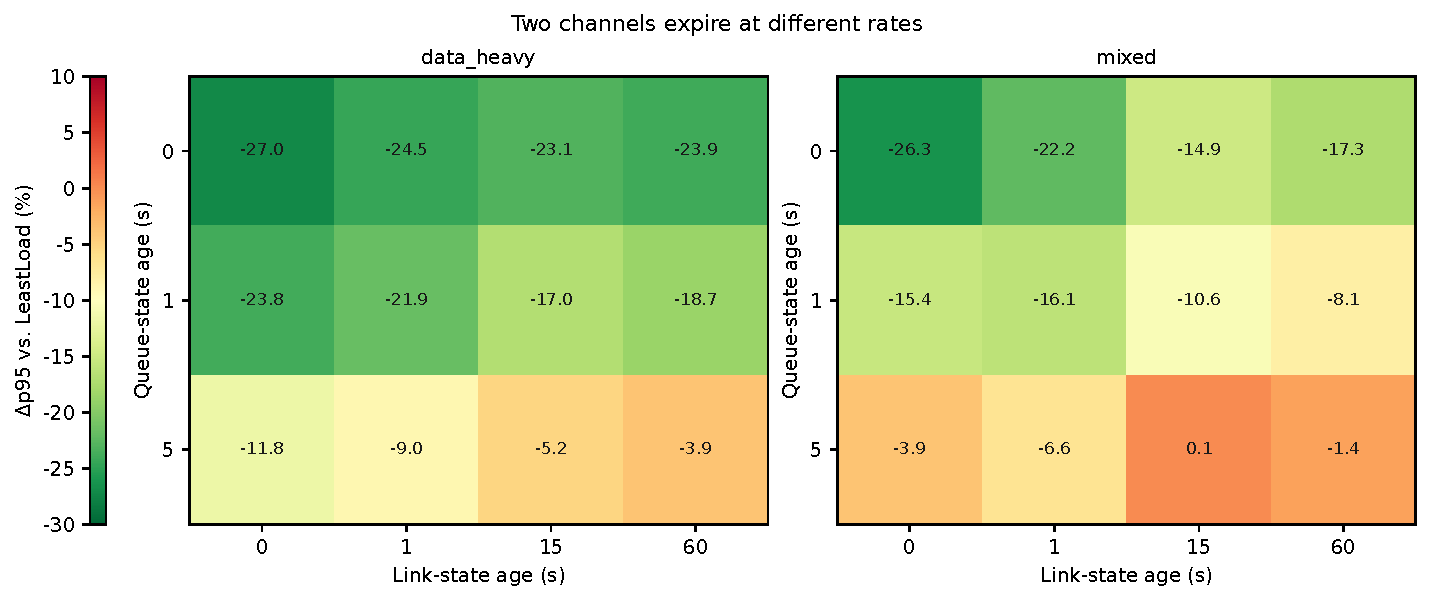
\includegraphics[width=\columnwidth]{fig_staleness_2d}
\caption{Joint staleness grid: benefit of the network-aware score relative to the network-blind
baseline as a function of link-state age (columns) and queue-state age (rows), on the volatile
network. Moving right costs little; moving down is expensive.}
\label{fig:staleness2d}
\end{figure}
We sweep queue age and link age \emph{jointly} (grid $\{0,1,5\}\,\text{s} \times
\{0,1,15,60\}\,\text{s}$, ten seeds, volatile network, since static networks make link age
exactly ineffective). Table~\ref{tab:staleness2d} and Fig.~\ref{fig:staleness2d} give the result. Two readings matter.

\begin{table}[t]
\centering
\caption{Joint staleness grid (synthetic, 10 seeds, NetworkAware2 vs LeastLoad, $\Delta$p95 in
\%). Rows: queue age; columns: link age. Reading down a column isolates link age; reading across
a row isolates queue age.}
\label{tab:staleness2d}
\small
\begin{tabular}{@{}lrrrr@{}}
\toprule
\multicolumn{1}{c}{} & \multicolumn{4}{c}{link age} \\
\cmidrule(lr){2-5}
queue age & \SI{0}{\second} & \SI{1}{\second} & \SI{15}{\second} & \SI{60}{\second} \\
\midrule
\multicolumn{5}{@{}l}{\emph{data-heavy}}\\
\SI{0}{\second}  & $-27$ & $-25$ & $-23$ & $-24$ \\
\SI{1}{\second}  & $-24$ & $-22$ & $-17$ & $-19$ \\
\SI{5}{\second}  & $-12$ & $-9$  & $-5$  & $-4$  \\
\midrule
\multicolumn{5}{@{}l}{\emph{mixed}}\\
\SI{0}{\second}  & $-26$ & $-22$ & $-15$ & $-17$ \\
\SI{1}{\second}  & $-15$ & $-16$ & $-11$ & $-8$  \\
\SI{5}{\second}  & $-4$  & $-7$  & $0$   & $-1$  \\
\bottomrule
\end{tabular}
\end{table}

First, \textbf{link state barely expires}. Holding the queue fresh, moving the link snapshot from
\SI{0}{\second} to \SI{60}{\second} leaves $89\%$ of the benefit for data-heavy traffic
($-27\%\rightarrow-24\%$) and $65\%$ for mixed ($-26\%\rightarrow-17\%$). This is not an
artifact of the static control: these cells are on the volatile network.

Second, \textbf{queue state expires fast, and the two compose}. Holding the link fresh, going
from \SI{0}{\second} to \SI{5}{\second} of queue age costs $56\%$ of the benefit for mixed
($-26\%\rightarrow-4\%$) and $56\%$ for data-heavy ($-27\%\rightarrow-12\%$). The two impairments
compound: with both channels old ($5\,\text{s}/60\,\text{s}$) the benefit is $-4\%$ (data-heavy)
and $-1\%$ (mixed), i.e.~smaller than either impairment alone would predict.
Comparing the channels at equal age is not meaningful: \emph{five seconds} of queue age destroys
$56$--$85\%$ of the benefit, whereas \emph{sixty seconds} of link age destroys only
$11$--$35\%$. Fitting a single exponential to each channel is not something two points per
channel supports, but the ordering is unambiguous and large: the queue channel's effective time
constant is roughly an order of magnitude (or more) smaller than the link channel's.

\paragraph{Why.} The two observables differ in what they are made of. A link's \emph{bandwidth}
is a slowly varying physical property, so even an old link snapshot still ranks workers almost
correctly on the structural part; only the congestion part is perishable. A compute queue has no
such structural component: it is entirely a statement about ``right now'', and it becomes wrong
at the rate the system's load changes. This observation is what makes the published
``telemetry delayed by \SI{60}{\second} does not matter'' finding \cite{aegis} both reproducible
and incomplete: the quantity swept was the slow-expiring channel.

\subsection{Latency and averaging are different distortions}
Real monitoring usually reports a \emph{time average} rather than an instantaneous value
(\texttt{avg\_over\_time} over the scrape interval), and a smoothing window is a different defect
from a lag: a lag makes the router react late, whereas averaging hides the very spike the router
is currently inside. We sweep the window independently of the lag (lag $=0$), for each channel.

Averaging inflates \emph{absolute} latency substantially and roughly equally for both policies:
a \SI{30}{\second} queue window moves p95 from \SI{46.2}{\second} to \SI{65.2}{\second} for the
network-aware policy and from \SI{139.6}{\second} to \SI{211.1}{\second} for the network-blind
baseline ($+41\%$ and $+51\%$; mixed/degraded: $+44\%$ and $+52\%$; mixed/unstable: $+46\%$ and
$+35\%$). The \emph{relative} advantage, however, moves much less: on the static network it is
essentially unchanged ($-67.0\%\rightarrow-69.1\%$ for data-heavy, $-71.7\%\rightarrow-69.1\%$
for mixed), and on the volatile network it erodes only moderately
($-20.4\%\rightarrow-14.4\%$ for mixed). Contrast this with the same amount of pure lag, which
at \SI{5}{\second} on the queue channel collapses the benefit to $-4\%$. In other words:
\textbf{for this system, being shown a smoothed average is far less damaging than being shown a
stale value}, which inverts the intuition that ``any loss of freshness is equally bad''. We
report the window channel separately for exactly this reason, and we note that the metric a real
monitoring stack reports---window length, scrape interval, and export delay---determines which of
the two distortions dominates.
